%----------------------------------------------------------
\def\notedate{2022.10.29}
\def\currentauthor{Василян А.Р. (РК6-73Б)}
%----------------------------------------------------------
\notestatement{rndhpcdsl}{Практическое ознакомление с Django и Docker}

%---------------------------------------------------------
На рисунке~\ref{picture1} представлено дерево проекта.
\begin{figure}[!ht]
  \centering
  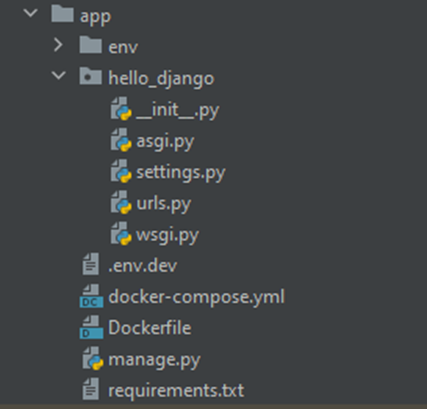
\includegraphics[scale=0.8]{ResearchNotes/rndhpc_not_gui_2022_10_29/picture1.png}
  \caption{Содержание проекта}
  \label{picture1}
\end{figure}

\begin{description}
	\item[\textsf{settings.py}] Файл содержит в себе все настройки проекта. Здесь регистрируются приложения, задаётся размещение статичных файлов, настройки базы данных и т.д. 
	\item[\textsf{urls.py}] Файл задаёт ассоциации url адресов с представлениями. 
	\item[\textsf{wsgi.py}] Используется для определения связи между Django приложением и веб-сервером.
	\item[\textsf{manage.py}] Используется для создания приложений, работы с базами данных и для запуска отладочного сервера.
\end{description}

	Был создан \textsf{Dockerfile} в каталоге проекта. Содержимое \textsf{Dockerfile} представлено в листинге~\ref{dockerfile}.

\begin{lstlisting}[frame=single,label={dockerfile},caption={Dockerfile},language={docker}] 
# pull official base image
FROM python:3.9.6-alpine

# set work directory
WORKDIR /usr/src/app

# set environment variables
ENV PYTHONDONTWRITEBYTECODE 1
ENV PYTHONUNBUFFERED 1

# install psycopg2 dependencies
RUN apk update \
    && apk add postgresql-dev gcc python3-dev musl-dev

# install dependencies
RUN pip install --upgrade pip
COPY ./requirements.txt .
RUN pip install -r requirements.txt

# copy project
COPY . .
\end{lstlisting}

	В \textsf{Dockerfile} описана последовательность команд, которые надо выполнить. На основе этого файла будет создан образ (\textsf{docker image}). Вначале указан образ на котором будем основываться. В нашем случае python 3.9. Устанавливается рабочая директория в контейнере с помощью \textsf{WORKDIR}. Далее устанавливаются переменные окружения:

\begin{enumerate}
	\item \textsf{PYTHONDONTWRITEBYTECODE} означает, что \textsf{Python} не будет пытаться создавать файлы \textsf{.pyc};
	\item \textsf{YTHONUNBUFFERED} гарантирует, что вывод консоли выглядит знакомым и не буферизируется Docker.
\end{enumerate}
	Затем команды для установки соответствующих пакетов, необходимых для \textsf{Psycopg2}. Из директории, где находится \textsf{Dockerfile}, копируется файл зависимостей \textsf{requirements.txt} в рабочую директорию контейнера. Далее с помощью команды \textsf{RUN} исполняются перечисленные в ней команды, что приводит к установкам зависимостей. Затем копируется вся дериктория проекта в контейнер.
	Был создан файл \textsf{docker-compose.yml} (листинг ~\ref{docker-compose}). \textsf{docker-compose} позволяет управлять многоконтейнерностью. То есть можно запустить сразу несколько контейнеров, которые будут работать между собой. В нашем случае мы создаем контейнер с базой данных \textsf{db} и наш основной контейнер \textsf{web}.
\begin{lstlisting}[frame=single, label={docker-compose}, caption={docker-compose.yml}, language={docker-compose}] 
version: '3.8'

services:
  web:
    build: .
    command: python manage.py runserver 0.0.0.0:8000
    volumes:
      - .:/usr/src/app/
    ports:
      - 8000:8000
    env_file:
      - .env.dev
    depends_on:
      - db
  db:
    image: postgres:13.0-alpine
    volumes:
      - postgres_data:/var/lib/postgresql/data/
    environment:
      - POSTGRES_USER=hello_django
      - POSTGRES_PASSWORD=hello_django
      - POSTGRES_DB=hello_django_dev

volumes:
# чтобы при работе контейнера сохранялись данные
  postgres_data:
\end{lstlisting}

	В самом начале указывается версия \textsf{docker-compose}. Далее указываются \textsf{services} (контейнеры). 
\begin{enumerate}
	\item \textsf{web}. Сбор проекта (\textsf{build}) делается на основе \textsf{Dockerfile} ("\textsf{.}" Значит, что он в той же директории, что и \textsf{docker-compose}). Далее указывается команда для запуска сервера. Указываем \textsf{volumes}, что значит, что всё из директории, где находится \textsf{docker-compose}, используется в контейнере. Далее указываются порты (сервер \textsf{Django} запускается в контейнере на порте \textsf{8000} и этот порт перебрасывается на нашу хост машину). И в конце сервиса \textsf{web} указывается зависимость от сервиса \textsf{db}, то есть \textsf{web} не сможет работать без \textsf{db}.
	\item \textsf{db}. Выбирается образ \textsf{postgres}. Далее указываются volumes, чтобы сохранять наши данные. Так же настраиваются переменные среды.
\end{enumerate}
	Команды, представленные на листинге ~\ref{settings1}, позволяют нам получить переменные окружения записанные в файл \textsf{.env.dev} (листинг ~\ref{.env.dev}) и записать их в переменные в файле проекта \textsf{settings.py}.

\begin{lstlisting}[frame=single, label={settings1}, caption={Обновлённые переменные в \textsf{settings.py}}, language=Python] 
SECRET_KEY = os.environ.get("SECRET_KEY")

DEBUG = int(os.environ.get("DEBUG", default=0))

ALLOWED_HOSTS = os.environ.get("DJANGO_ALLOWED_HOSTS").split(" ")
\end{lstlisting}

	\textsf{SECRET_KEY} — это секретный ключ, который используется Django для поддержки безопасности сайта.
	\textsf{DEBUG}. Включает подробные сообщения об ошибках, вместо стандартных \textsf{HTTP} статусов ответов. Должно быть изменено на \textsf{False} на сервере, так как эта информация очень много расскажет взломщикам.
	\textsf{ALLOWED_HOSTS} — это список хостов/доменов, для которых может работать текущий сайт.
	Так же в \textsf{setings.py} были обновлены настройки базы данных (листинг ~\ref{settings2}) на основе переменных окружения, определённых в \textsf{.env.dev}.

\begin{lstlisting}[frame=single, label={settings2}, caption={Обновлённые переменные в \textsf{settings.py}}, language={json}] 
DATABASES = {
    "default": {
        "ENGINE": os.environ.get("SQL_ENGINE", "django.db.backends.sqlite3"),
        "NAME": os.environ.get("SQL_DATABASE", BASE_DIR / "db.sqlite3"),
        "USER": os.environ.get("SQL_USER", "user"),
        "PASSWORD": os.environ.get("SQL_PASSWORD", "password"),
        "HOST": os.environ.get("SQL_HOST", "localhost"),
        "PORT": os.environ.get("SQL_PORT", "5432"),
    }
}
\end{lstlisting}

\begin{lstlisting}[frame=single, label={.env.dev}, caption={Содержимое файла \textsf{.env.dev}}, language={aINIExample}] 
DEBUG=1
SECRET_KEY=foo
DJANGO_ALLOWED_HOSTS=localhost 127.0.0.1 [::1]
SQL_ENGINE=django.db.backends.postgresql
SQL_DATABASE=hello_django_dev
SQL_USER=hello_django
SQL_PASSWORD=hello_django
SQL_HOST=db
SQL_PORT=5432
\end{lstlisting}

	На рисунке ~\ref{picture2} изображено приветственное окно \textsf{Django}, что свидетельствует о том, что проект \textsf{Django} был успешно настроен.

\begin{figure}[!ht]
  \centering
  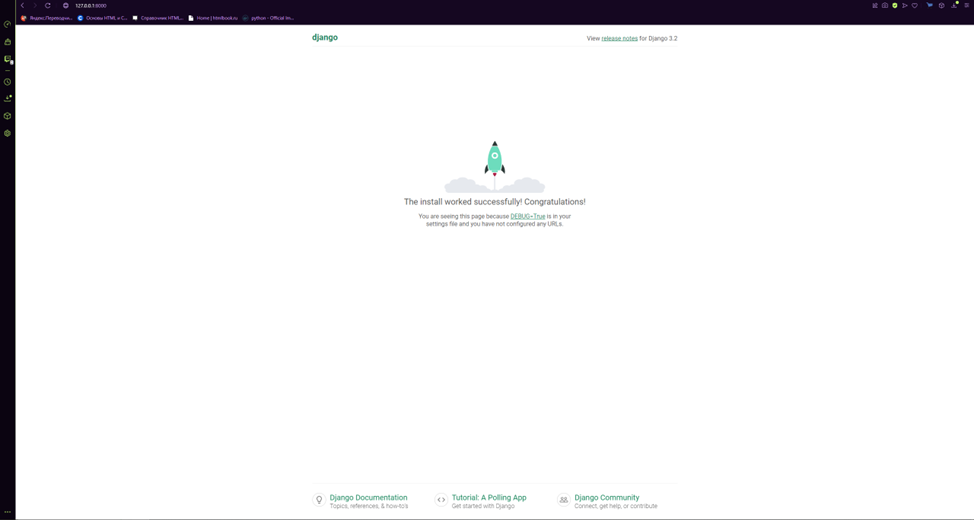
\includegraphics[scale=0.8]{ResearchNotes/rndhpc_not_gui_2022_10_29/picture2.png}
  \caption{Окно приветствия}
  \label{picture2}
\end{figure}

	Входим в контейнер и создаём суперпользователя (рисунок ~\ref{picture3}).
\begin{figure}[!ht]
  \centering
  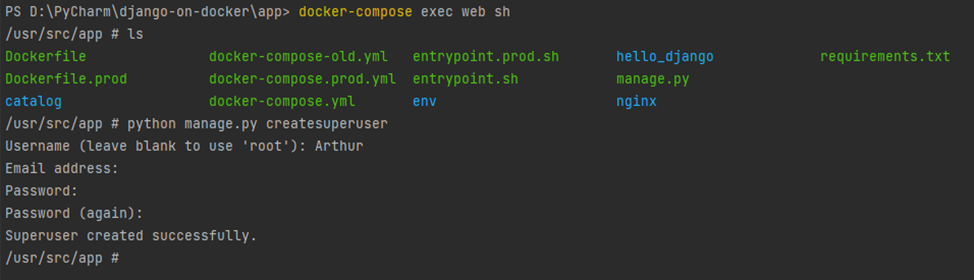
\includegraphics[scale=0.8]{ResearchNotes/rndhpc_not_gui_2022_10_29/picture3.png}
  \caption{Создание суперпользователя}
  \label{picture3}
\end{figure}

	Переходим по адресу \textsf{127.0.0.1:8000/admin/} и вводим имя и пароль суперпользователя. Вход выполнен (рисунок ~\ref{picture4}).
\begin{figure}[!ht]
  \centering
  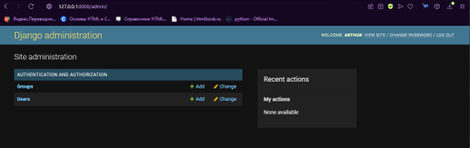
\includegraphics[scale=0.8]{ResearchNotes/rndhpc_not_gui_2022_10_29/picture4.png}
  \caption{Вход успешно выполнен}
  \label{picture4}
\end{figure}

	Проверка на создание таблиц по умолчанию на рисунке ~\ref{picture5}.
\begin{figure}[!ht]
  \centering
  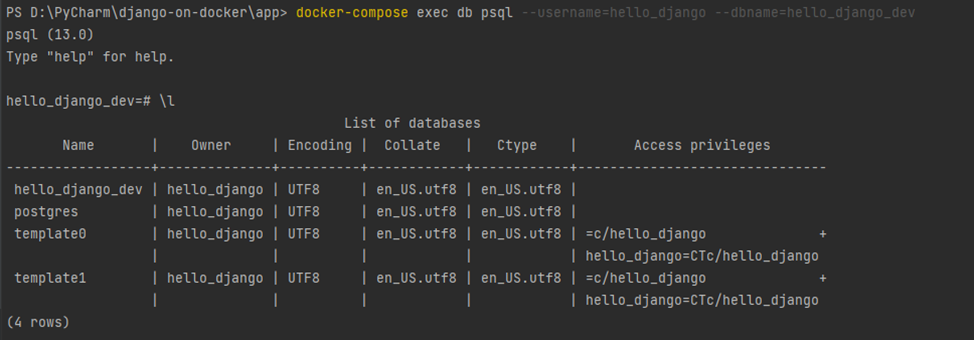
\includegraphics[scale=0.8]{ResearchNotes/rndhpc_not_gui_2022_10_29/picture5.png}
  \caption{Проверка таблиц}
  \label{picture5}
\end{figure}
%----------------------------------------------------------
% Атрибуты задачи
\noteattributes{}
%----------------------------------------------------------
